\section{Discussion}
In this section we discuss the implications and insights provided by the results presented in Theorems~\ref{cmt2mn} and ~\ref{polthe}.
\subsection{On Error Terms}
\begin{itemize}
\item The error bounds in the main results (Theorems~\ref{cmt2mn} and \ref{polthe}) contain two factors namely
\begin{enumerate}
\item $\min_{r\in \R^k} ||J^*-\Phi r||_{\mn}$,
\item $||\Gamma J^*-\hg J^*||_{\mn}$.
\end{enumerate}
The first factor is related to the best possible approximation that can be achieved with the chosen feature matrix $\Phi$. This term is inherent to the ALP formulation and it appears in the bounds provided by \cite{ALP}.\\
The second factor is related to constraint approximation and is completely defined in terms of $\Phi$, $W$ and $T$, and does not require knowledge of stationary distribution of the optimal policy. It makes intuitive sense since given that $\Phi$ approximates $J^*$, it is enough for $W$ to depend on $\Phi$ and $T$ without any additional requirements.
\item Unlike the result in \cite{CS} which holds only for a specific RLP formulated under ideal assumptions, our bounds hold for any GRLP and as a result for any given RLP. Another interesting feature of our result is that it holds with probability $1$. 
\item A salient feature of the ALP formulation is the use of Lyapunov functions to control/shape the error across the states based on their relative importance. Since the error bounds are in a modified $L_\infty$-norm, the GRLP framework retains this salient feature of the ALP.
\end{itemize}
The fact that both the prediction and control problems can be addressed by the GRLP makes it a complete ADP method, and by addressing the constraint approximation, the GRLP framework is an important addition to the theory of ALP.
\subsection{On Constraint Reduction and Approximation}
We claim the following based on the error bounds that we derived for the GRLP.\\
{Claim $1$)} It is not always necessary to sample constraints according to the stationary distribution of the optimal policy.\\
{Claim $2$)} Constraint approximation is not only restricted to constraint sampling but also can be extended to include linear approximation of the constraints.\\
The following result (Theorem~\ref{st}) supports Claim~$1$ in the above.\\
\textbf{Main Result~$3$: On Constraint Sampling}\\
The error term $\etmn$ gives new insights into constraint sampling. 
\begin{comment}
Before we state our result, we define what we call a \emph{constraint sampling} matrix
\begin{definition}
Let the index set $\I=\{i_1,\ldots,i_m\}$ ( $1\leq i_1<\ldots<i_m\leq n\times d$) denote the constraints to be sampled. We call the $nd\times m$ matrix $W$ to be the corresponding \emph{constraint sampling} matrix and is defined as
\begin{align}
W(i,j)&=1, \mb\text{if}\mb q_i=j\nn\\
&=0, \mb\text{otherwise}
\end{align}
\end{definition}
\end{comment}
\begin{theorem}\label{st}
Let $s\in S$ be a state whose constraint was sampled. Then
\begin{align}\label{sampexp}
|\Gamma J^*(s)-\hg J^*(s)|<|\Gamma J^*(s)-J^*(s)|.
\end{align}
\end{theorem}
\begin{proof}
Let $r_{e_s}$ and $\hat{r}_{e_s}$ be solutions to the linear programs in \eqref{lubplp} and \eqref{alubplp} respectively for $c=e_s$ and $J=J^*$. It is easy to note that $r_{e_s}$ is feasible for the linear program in \eqref{alubplp} for $c=e_s$ and $J^*$, and hence it follows that $(\Phi r_{e_s})(s)\geq (\Phi \hat{r}_{e_s})(s)$. However, since all the constraints with respect to state $s$ have been sampled we know that $(\Phi \hat{r}_{e_s})(s)\geq J^*$. The proof follows from noting that $(\Gamma J^*)(s)=(\Phi r_{e_s})(s)$ and $\hg J^*(s)=(\Phi \hat{r}_{e_s})(s)$.
\end{proof}\\
The expression in \eqref{sampexp} in Theorem~\ref{st} says that the additional error $|\Gamma J^*(s) -\hg J^*(s)|$ due to constraint sampling is less than the original projection error $|\Gamma J^*(s)-J^*(s)|$ due to function approximation. This means that for the RLP to perform well it is enough to retain those states for which the linear function approximation via $\Phi$ is known to perform well. The modified $L_\infty$ norm in \eqref{finalbnd} comes to our rescue to control the error due to those states that are not sampled. Thus the sampling distribution need not be the stationary distribution of the optimal policy as long as it samples the \emph{important} states, an observation that might theoretically explain the empirical successes of the RLP \cite{ALP,CST,SALP}.\\
To understand the implication of Claim~$2$ we need to look at the Lagrangian of the ALP and GRLP in \eqref{lag} and \eqref{lag2} respectively, i.e., 
\begin{align}\label{lag}
\tilde{L}(r,\lambda)=c^\top \Phi r+\lambda^\top (T\Phi r-\Phi r), \\ \label{lag2}\hat{L}(r,q)=c^\top \Phi r+q^\top W^\top (T\Phi r-\Phi r).
\end{align}
The insight that the GRLP is a linear function approximation of the constraints (i.e., the Lagrangian multipliers) can be obtained by noting that $ Wq\approx \lambda$ in \eqref{lag2}. Note that while the ALP employs LFA in its objective function (i.e., use of $\Phi r$), the GRLP employs linear approximation both in the objective function ($\Phi r$) as well as the constraints (use of $W$). Further, $W$ can be interpreted as the feature matrix that approximates the Lagrange multipliers as $\lambda\approx Wq$, where $\lambda \in \R^{nd}, r\in \R^m$. One can show \cite{dolgov} that the optimal Lagrange multipliers are the discounted number of visits to the ``state-action pairs'' under the optimal policy $u^*$, i.e., 
\begin{align}
\lambda^*(s,u^*(s))&=\big(c^\top(I-\alpha P_{u^*})^{-1}\big)(s)\nn\\
				&= \big(c^\top(I+\alpha P_{u^*}+\alpha^2 P_{u^*}^2+\ldots)\big)(s),\nn\\
			\lambda^*(s,a)&=0, \forall a \neq u^*(s),\nn
\end{align}
where $P_{u^*}$ is the probability transition matrix with respect to the optimal policy. Even though we might not have the optimal policy $u^*$ in practice, the fact that $\lambda^*$ is a probability distribution and that it is a linear combination of $\{P_{u^*},P^2_{u^*},\ldots\}$ hints at the kind of features that might be useful for the $W$ matrix.\\
\subsection{Numerical Illustration}
We take up an example in the domain of controlled queues from \cite{ALP} for which the ALP has been known to work well. For this domain, we make use of our results and observations to select various useful $W$ matrices and present their performance.\\
The queuing system consists of $n=10^4$ states and $d=4$ actions. We chose $n=10^4$ because it was possible to solve both the GRLP and the exact LP (the latter with significant effort) so as to enumerate the approximation errors. We hasten to mention that while we could run the GRLP for queuing systems with $n>10^4$ without much computational overhead, solving the exact LP was not possible for $n>10^4$ as a result of which the approximation error could not be computed.\\
\textbf{Queuing Model:}
The queuing model used here is similar to the one in Section~$5.2$ of \cite{ALP}. We consider a single queue with arrivals and departures. The state of the system is the queue length with the state space given by $S=\{0,\ldots,n-1\}$, where $n-1$ is the buffer size of the queue. The action set $A=\{1,\ldots,d\}$ is related to the service rates. We let $s_t$ denote the state at time $t$. The state at time $t+1$ when action $a_t \in A $ is chosen is given by $s_{t+1}= s_{t}+1$ with probability $p$, $s_{t+1}= s_{t}-1$ with probability $q(a_t)$ and $s_{t+1}= s_t$, with probability $(1-p-q(a_t))$. For states $s_t=0$ and $s_t=n-1$, the system dynamics is given by 	$s_{t+1}= s_{t}+1$ with probability $p$ when $s_t=0$ and $s_{t+1}=s_t-1$ with probability $q(a_t)$ when $s_t=n-1$.
The service rates satisfy $0<q(1)\leq \ldots\leq q(d)<1$ with $q(d)>p$ so as to ensure `stabilizability' of the queue. The reward associated with the action $a \in A$ in state $s\in S$ is given by $g_a(s)=-(s+60q(a)^3)$.\\
\textbf{Choice of $\Phi:$} We make use of polynomial features in $\Phi$ (i.e., $1,s,\ldots,s^{k-1}$) since they are known to work well for this domain \cite{ALP}. This takes care of the term $||J^*-\Phi r^*||_\infty$ in \eqref{finalbnd}. \\
\textbf{Selection of $W$:} For our experiments, we choose two contenders for the $W$-matrix and compare them with the ideal sampling matrix $W_i$ (\cite{CS}) and random positive matrix $W_r$. Our choices of the $W$ matrix are as below.\\
{$\mathbf{(i)}$} $W_c$- matrix that corresponds to sampling according to $c$. This is justified by the insights obtained from Theorem~\ref{st} on the error term $\et$, i.e., the idea of selecting the important states.\\
{$\mathbf{(ii)}$} $W_a$ state-aggregation matrix, a heuristic derived using the fact that $\lambda^*$ is a linear combination of $\{P_{u^*},P^2_{u^*},\ldots\}$. Our choice of the $W_a$ matrix to correspond to aggregation of near by states is motivated by the observation that $P^n$ captures $n^{th}$ hop connectivity/neighborhood information.
The aggregation matrix $W_a$ is defined as below: $\forall i=1,\ldots,m$,
\begin{align}\label{wdes}
W_a(i,j)&=1, \mb\forall j\mb\text{s.t}\mb j=(i-1)\times\frac{n}{m}+k+(l-1)\times n, \nn\\&\mb\quad\quad k=1,\ldots,\frac{n}{m}, l=1,\ldots,d,\nn\\
&=0,\mb\text{otherwise}.
\end{align}
We ran our experiments on a moderately large queuing system denoted by $Q_L$ with $n=10^4$ and $d=4$ with $q(1)=0.2$, $q(2)=0.4$, $q(3)=0.6$, $q(4)=0.8$, $p=0.4$ and $\alpha=0.98$. We chose $k=4$ (i.e., we used $1, s,s^2$ and $s^3$ as basis vectors) and we chose $W_a$ \eqref{wdes}, $W_c$, $W_i$ and $W_r$ with $m=50$. We set $c(s)=(1-\zeta) \zeta^s, \mb\forall s=1,\ldots,9999$, with $\zeta=0.9$ and $\zeta=0.999$ respectively. The results in Table~\ref{pref} show that the performance exhibited by $W_a$ and $W_c$ is better by several orders of magnitude over `random' in the case of the large system $Q_L$ and is closer to the ideal sampler $W_i$. Also note that a better performance of $W_a$ and $W_c$ in the larger system $Q_L$ tallies with a lower value of $\et$ in the smaller system $Q_S$.
\FloatBarrier
\begin{table}[H]
%\resizebox{\columnwidth}{!}{
\begin{tabular}{|c|c|c|c|c|}\hline
Error Terms&	$W_i$&	$W_c$& $W_a$& $W_r$ \\\hline
$||J^*-\hj||_{1,c}$ for $\zeta=0.9$& $32$&	$32$& $220$& $5.04\times 10^4$ \\\hline
$||J^*-\hj||_{1,c}$ for $\zeta=0.999$& $110$&	$180.5608$& $82$& $1.25\times 10^7$ \\\hline
\end{tabular}
%}
\caption{Shows values of Error Terms for $Q_L$.}
\label{pref}
\end{table}

\FloatBarrier
\begin{table}[H]
%\resizebox{\columnwidth}{!}{
\begin{tabular}{|c|c|c|c|}\hline
Performance Metric&	$W_i$&	$W_c$& $W_a$ \\\hline
$||J_{\hu}||_{1,c}$ for $\zeta=0.9$& $-441.25$&	$-450.59$& $-446.49$ \\\hline
$||J_{\hu}||_{1,c}$ for $\zeta=0.999$& $-2.0611e+04$&	$-2.0611e+04$& $-2.0612e+04$ \\\hline
\end{tabular}
%}
\caption{Shows performance metrics for $Q_L$. Here $||J^*||_{1,c}=-439.26$ for $\zeta=0.9$ and $||J^*||_{1,c}=-2.0603e+04$ for $\zeta=0.999$   and a random policy yields a total reward of $-1.2661e+03
$.}
\label{pref}
\end{table}
Empirical evidence for the performance of RLP with various sampling distributions can also be found in \cite{CST,CS}.
\subsection{Reinforcement Learning}
Reinforcement Learning (RL) algorithms are useful in scenarios where the system is available in the form of a simulator or only samples can be obtained via direct interaction. In particular, in the RL setting, the model parameters $g$ and $P$ are not known explicitly and the underlying MDP needs to be solved by using sample trajectories. In short, RL algorithms are sample trajectory based solution schemes for solving MDPs whose model information is not known. RL methods learn by filtering out the noisy sample via stochastic approximation and they also employ function approximation in order to handle MDPs with large number of states. Most RL algorithms are sample trajectory based extensions of ADP methods.\\
The RL extension of the ALP formulation has been applied to the optimal stopping problem in \cite{ALP-Bor}. Function approximation is employed to approximate the square root of the Lagrange multipliers. However, since the approximation is not linear, convergence of the resulting RL algorithm cannot be guaranteed. Our results theoretically justify linear function approximation of the Lagrange multipliers, an immediate implication of which is that the RL extension of the ALP can be guaranteed to converge if the updates in \cite{ALP-Bor} use LFA for the Lagrange multipliers instead of a non-linear approximator.
\begin{comment}
We now consider the mountain car example. The problem is to make an under-powered car climb a one-dimensional hill (Fig.~\ref{mcar}), whose position $x$ lies in the interval $[-1.2,0.5]$. There are $3$ actions available to the car, i.e., $A=\{0,1,2\}$. Here $a=0$ and $a=2$ correspond to accelerating to the left and the right respectively. Further, $a=1$ corresponds to no acceleration. The velocity $y$ is limited to $[-0.07,0.07]$. The dynamics is given by
\begin{align}
y_{t+1}&=y_t+0.001 (a_t-1)-0.0025 \cos(3x_t),\\
x_{t+1}&=x_t+y_t.
\end{align}
The state space is continuous with $S=[-1.2,0.5]\times[-0.07,0.07]$ and the state is given by $s=(x,y), x\in [-1.2,0.5], y \in [-0.07,0.07]$. The goal-state is reached once the car crosses the position $x\geq 0.5$. The reward in the goal-state is $100$ and the reward is $0$ in all the other states. 
\FloatBarrier
\begin{figure}[H]
\begin{center}
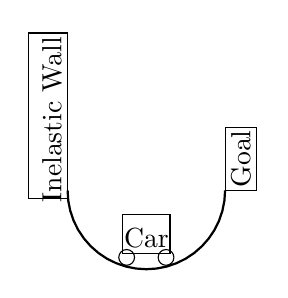
\begin{tikzpicture}
\draw [black,thick,domain=180:360] plot ({cos(\x)}, {sin(\x)});
\node [rotate=90] at (-1.2,0.9) { Inelastic Wall};
\draw (-1.5,-.1) rectangle (-1,2.0);
\node[] at (0,-0.6) { Car};
\draw (-0.3,-0.8) rectangle (0.3,-0.3);
\draw (1,0.0) rectangle (1.4,0.8);

\draw[] (-0.25,-0.85) circle(0.1);
\draw[] (0.25,-0.85) circle(0.1);
\node [rotate=90] at (1.2,0.4) { Goal};
\end{tikzpicture}
\end{center}
\caption{Mountain Car}
\label{mcar}
\end{figure}


\begin{figure}
\centering
\includegraphics[scale=1.0]{careps1.eps}
\caption{Mountain Car}
\label{mcar}
\end{figure}
\end{comment}

